\documentclass[12pt, a4paper]{article}

% ── Core Packages ─────────────────────────────────────────────────────
\usepackage[top=2.5cm, bottom=2.5cm, left=2.5cm, right=2.5cm]{geometry}
\usepackage{fontenc}
\usepackage{inputenc}
\usepackage[sfdefault]{roboto}
\usepackage{titlesec}
\usepackage{booktabs}
\usepackage{array}
\usepackage{tabularx}
\usepackage{hyperref}
\usepackage{xcolor}
\usepackage{fancyhdr}
\usepackage{enumitem}
\usepackage{parskip}
\usepackage{tcolorbox}
\usepackage{amsmath}
\usepackage{microtype}
\usepackage{graphicx}
\usepackage{tikz}
\usepackage{mdframed}
\usepackage{colortbl}
\usepackage{multirow}
\usepackage{setspace}

\tcbuselibrary{skins, breakable}
\usetikzlibrary{calc}

% ── Colors ────────────────────────────────────────────────────────────
\definecolor{mainblue}{RGB}{41, 128, 185}
\definecolor{darkblue}{RGB}{26, 26, 46}
\definecolor{lightgray}{RGB}{245, 246, 248}
\definecolor{midgray}{RGB}{150, 150, 150}
\definecolor{successgreen}{RGB}{39, 174, 96}
\definecolor{warnorange}{RGB}{243, 156, 18}
\definecolor{tableheader}{RGB}{44, 62, 80}
\definecolor{accentlight}{RGB}{214, 234, 248}

% ── Hyperlinks ────────────────────────────────────────────────────────
\hypersetup{
  colorlinks=true,
  linkcolor=mainblue,
  urlcolor=mainblue,
  pdftitle={EV Charging Demand Prediction - Milestone 1},
  pdfauthor={Applied ML Team}
}

% ── Header / Footer ───────────────────────────────────────────────────
\pagestyle{fancy}
\fancyhf{}
\renewcommand{\headrulewidth}{0pt}
\fancyhead[L]{%
  
\begin{tikzpicture}[remember picture, overlay]
    \draw[mainblue, line width=1.5pt] (0,0) -- (\textwidth,0);
  \end{tikzpicture}%
  \vspace{2pt}\small\color{midgray}\textbf{EV Charging Demand Prediction}
}
\fancyhead[R]{\small\color{midgray} Milestone 1}
\fancyfoot[C]{\small\color{midgray}\thepage}
\fancyfoot[L]{\small\color{midgray} Applied Machine Learning}

% ── Section Styling ───────────────────────────────────────────────────
\titleformat{\section}{
  \large\bfseries\color{darkblue}
}{\textcolor{mainblue}{\thesection}}{0.6em}{}[
  \vspace{-0.4em}\textcolor{mainblue}{\rule{\linewidth}{1.5pt}}\vspace{0.2em}
]

\titleformat{\subsection}{
  \normalsize\bfseries\color{darkblue}
}{\textcolor{mainblue}{\thesubsection}}{0.5em}{}

\titlespacing*{\section}{0pt}{2em}{0.8em}
\titlespacing*{\subsection}{0pt}{1.2em}{0.4em}

% ── tcolorbox Styles ──────────────────────────────────────────────────
\tcbset{
  highlight/.style={
    enhanced,
    colback=successgreen!8,
    colframe=successgreen!60!black,
    fonttitle=\bfseries\small,
    boxrule=0pt, leftrule=4pt,
    arc=3pt,
    left=8pt, right=8pt, top=6pt, bottom=6pt
  },
  warning/.style={
    enhanced,
    colback=warnorange!8,
    colframe=warnorange!70!black,
    fonttitle=\bfseries\small,
    boxrule=0pt, leftrule=4pt,
    arc=3pt,
    left=8pt, right=8pt, top=6pt, bottom=6pt
  }
}

% ── List Styling ──────────────────────────────────────────────────────
\setlist[itemize]{
  leftmargin=1.5em,
  itemsep=0.3em,
  label=\textcolor{mainblue}{$\bullet$}
}
\setlist[enumerate]{leftmargin=1.5em, itemsep=0.3em}

% ══════════════════════════════════════════════════════════════════════
\begin{document}
% ══════════════════════════════════════════════════════════════════════

% ── COVER PAGE ────────────────────────────────────────────────────────
\begin{titlepage}
\thispagestyle{empty}

% Top accent bar
\begin{tikzpicture}[remember picture, overlay]
  \fill[darkblue] (current page.north west) rectangle +(\paperwidth, -3.5cm);
  \fill[mainblue] (current page.north west) ++(0,-3.5cm) rectangle +(\paperwidth, -0.5cm);
\end{tikzpicture}

\vspace*{1.2cm}

% Top bar text
{\color{white}\centering
  {\small\bfseries\MakeUppercase{Applied Machine Learning \quad\textperiodcentered\quad Term Project}}\\[0.3cm]
  {\footnotesize\color{accentlight}\MakeUppercase{Mid-Semester Submission \quad\textperiodcentered\quad Milestone 1}}
}

\vspace{3.5cm}

% Main title block
\centering
{%
  \fontsize{30}{38}\selectfont\bfseries\color{darkblue}
  Intelligent EV Charging\\[0.3em]
  Demand Prediction\\[0.3em]
  \&\\[0.3em]
  Agentic Infrastructure\\[0.3em]
  Planning
}

\vspace{0.8cm}
{\large\itshape\color{midgray} Milestone 1 --- Data Pipeline \& Machine Learning Modeling}

\vspace{1cm}
\textcolor{mainblue}{\rule{4cm}{1.5pt}}

\vspace{1.5cm}

% Team block
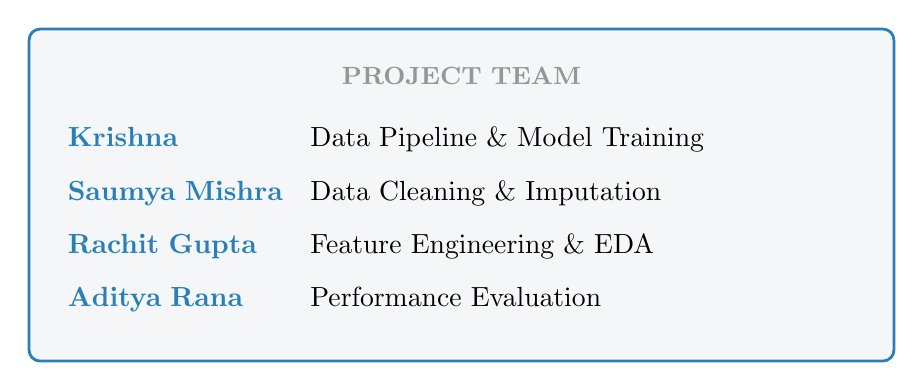
\begin{tikzpicture}
  \node[
    draw=mainblue,
    line width=1pt,
    fill=lightgray,
    rounded corners=4pt,
    inner sep=14pt,
    text width=10cm
  ] {
    \centering
    {\small\bfseries\color{midgray}\MakeUppercase{Project Team}}\\[8pt]
    \renewcommand{\arraystretch}{1.6}
    \begin{tabular}{@{}l@{\hspace{1em}}l@{}}
      \textcolor{mainblue}{\textbf{Krishna}}       & Data Pipeline \& Model Training \\
      \textcolor{mainblue}{\textbf{Saumya Mishra}} & Data Cleaning \& Imputation     \\
      \textcolor{mainblue}{\textbf{Rachit Gupta}}  & Feature Engineering \& EDA      \\
      \textcolor{mainblue}{\textbf{Aditya Rana}}   & Performance Evaluation          \\
    \end{tabular}
  };
\end{tikzpicture}

\vspace{1.5cm}

% Meta row
\begin{tikzpicture}
  \node[
    fill=darkblue,
    rounded corners=4pt,
    inner sep=10pt,
    text width=12cm,
    align=center
  ] {
    \color{white}\small
    \textbf{Submission:} Mid-Semester \quad
    \textcolor{accentlight}{\textperiodcentered} \quad
    \textbf{Framework:} Scikit-Learn
  };
\end{tikzpicture}

% Bottom accent bar
\begin{tikzpicture}[remember picture, overlay]
  \fill[darkblue] (current page.south west) rectangle +(\paperwidth, 1.5cm);
  \fill[mainblue] (current page.south west) ++(0,1.5cm) rectangle +(\paperwidth, 0.3cm);
\end{tikzpicture}

\end{titlepage}

% ── TABLE OF CONTENTS ─────────────────────────────────────────────────
\newpage
\tableofcontents
\newpage

% ── ABSTRACT ──────────────────────────────────────────────────────────
\begin{mdframed}[
  linecolor=mainblue,
  linewidth=1pt,
  backgroundcolor=lightgray,
  innerleftmargin=14pt,
  innerrightmargin=14pt,
  innertopmargin=12pt,
  innerbottommargin=12pt,
  roundcorner=4pt
]
{\centering\small\bfseries\color{midgray}\MakeUppercase{Abstract}\par\vspace{8pt}}
\noindent
The rapid adoption of electric vehicles (EVs) has introduced significant challenges
in managing load on power grids and optimizing charging infrastructure placement.
This report presents Milestone 1 of a two-phase AI-driven analytics system.
We construct an end-to-end machine learning pipeline that consolidates real-world
charging session data from three California stations (89,715 records), performs
systematic data cleaning and median imputation, engineers time-series and lag-based
features, and trains a Random Forest Regressor to predict EV charging demand.
The model achieves an R\textsuperscript{2} accuracy of \textbf{88.65\%} with a
Mean Absolute Error of \textbf{0.0192 kW}. The trained model is serialized for
integration into the Milestone 2 agentic planning system.
\end{mdframed}

% ── SECTION 1: INTRODUCTION ───────────────────────────────────────────
\section{Introduction}

Electric vehicles are transitioning from niche technology to mainstream transportation.
This shift places unprecedented and often unpredictable demand on the electrical grid.
Charging stations must be intelligently sited and operated, and grid operators require
accurate demand forecasts to avoid overloads and service degradation.

This project, developed under free-tier API constraints and open-source tooling,
proposes an end-to-end AI system addressing both predictive modeling (Milestone 1)
and agentic infrastructure planning (Milestone 2). The present report covers
Milestone 1 exclusively.

The primary objectives of Milestone 1 are:

\begin{itemize}
  \item Consolidate and synchronize multi-source charging station time-series data from three California locations.
  \item Perform rigorous cleaning, outlier inspection, and feature imputation.
  \item Engineer temporally-aware features including lag variables and rolling averages.
  \item Train and evaluate a supervised regression model for demand prediction.
  \item Serialize the trained model for downstream agentic use in Milestone 2.
\end{itemize}

% ── SECTION 2: DOMAIN BACKGROUND ─────────────────────────────────────
\section{Domain Background}

EV charging demand is a multi-variate time-series problem influenced by temporal
patterns (time-of-day, day-of-week), environmental conditions (weather), grid state
(stability index, availability), electricity pricing, and the concurrent number of
active charging sessions. Prior work demonstrates that tree-based ensemble models
such as Random Forests perform competitively against deep learning approaches when
appropriate lag features are constructed, particularly on shorter time horizons.

Our dataset derives from three real-world California charging stations (A, B, C),
providing geographic and operational diversity. California's leadership in EV adoption
makes it an ideal testbed for this research.

% ── SECTION 3: DATASET ────────────────────────────────────────────────
\section{Dataset Description}

\begin{table}[h!]
\centering
\caption{Dataset Summary After Consolidation}
\renewcommand{\arraystretch}{1.4}
\begin{tabularx}{\textwidth}{>{\bfseries}lX}
\toprule
\rowcolor{tableheader}
\color{white}Attribute & \color{white}Details \\
\midrule
Source Files      & Charging\_Station\_A\_Calif.csv, \_B\_Calif.csv, \_C\_Calif.csv \\
\rowcolor{lightgray}
Total Records     & 89,715 rows \\
Stations          & 3 (IDs: 0, 1, 2 --- California, USA) \\
\rowcolor{lightgray}
Temporal Coverage & Multi-month time-series (hourly granularity) \\
Target Variable   & EV Charging Demand (kW) \\
\rowcolor{lightgray}
Key Input Features & Date/Time, Weather Conditions, Electricity Price (\$/kWh), Grid Stability Index, Grid Availability, Number of EVs Charging \\
Missing Values    & Present; resolved via median imputation \\
\bottomrule
\end{tabularx}
\end{table}

% ── SECTION 4: METHODOLOGY ────────────────────────────────────────────
\section{Methodology}

\subsection{System Architecture Overview}

The end-to-end pipeline follows six sequential phases:

\vspace{0.5em}
\begin{center}
\small
\begin{tikzpicture}[node distance=0.4cm]
  \tikzstyle{box} = [rectangle, rounded corners=3pt, fill=darkblue, text=white,
                     font=\small\bfseries, inner sep=6pt, text width=2cm, align=center]
  \tikzstyle{arr} = [->, thick, color=mainblue]

  \node[box] (a) {Raw CSV\\(3 files)};
  \node[box, right=of a] (b) {Data\\Consolidation};
  \node[box, right=of b] (c) {Cleaning \&\\Imputation};
  \node[box, right=of c] (d) {Feature\\Engineering};
  \node[box, right=of d] (e) {Model\\Training};
  \node[box, right=of e] (f) {Evaluation \&\\Export};

  \draw[arr] (a) -- (b);
  \draw[arr] (b) -- (c);
  \draw[arr] (c) -- (d);
  \draw[arr] (d) -- (e);
  \draw[arr] (e) -- (f);
\end{tikzpicture}
\end{center}
\vspace{0.3em}
{\centering\small\itshape\color{midgray} Figure 1 --- End-to-end ML pipeline for Milestone 1.\par}

\subsection{Phase 1 --- Data Loading \& Consolidation \textnormal{\small\itshape(Krishna)}}

Three station CSV files were loaded using \texttt{pandas.read\_csv()}. A \texttt{Station\_ID}
column (0, 1, 2) was appended to preserve provenance. The \texttt{Date} and \texttt{Time}
columns were concatenated into a unified \texttt{Datetime} column and parsed with
\texttt{format=`mixed'} to tolerate heterogeneous date formats across stations. All
DataFrames were concatenated and sorted by \texttt{[Station\_ID, Datetime]}, yielding
a single chronologically-ordered dataset of \textbf{89,715 records}.

\subsection{Phase 2 --- Data Cleaning \& Imputation \textnormal{\small\itshape(Saumya Mishra)}}

The auxiliary \texttt{Datetime\_Str} column was dropped post-parsing. Missing numeric
values were filled using column-wise \textbf{median imputation}, which is robust to
the outliers visible in electricity price and grid stability distributions. The
categorical \texttt{Grid Availability} feature was binary-encoded:
\textit{Available = 1}, \textit{Unavailable = 0}.

Visual diagnostics included: (i) a null-value heatmap confirming no residual gaps
post-imputation; (ii) boxplots of key numeric features; (iii) a KDE histogram of the
target variable showing a right-skewed demand distribution; and (iv) a pie chart and
count plot for weather conditions and grid availability.

\subsection{Phase 3 --- Feature Engineering \& EDA \textnormal{\small\itshape(Rachit Gupta)}}

Temporal features extracted: \texttt{Hour} (0--23) and \texttt{DayOfWeek} (0--6)
capture intra-day and intra-week cyclical patterns. Two lag features,
\texttt{Demand\_Lag\_1} and \texttt{Demand\_Lag\_2}, encode demand at $t-1$ and $t-2$,
computed within each station group to prevent cross-station leakage. A
\texttt{Rolling\_Avg\_3h} feature captures recent short-term trend using a 3-step
rolling mean shifted by 1 to avoid data leakage. Rows with NaN values were then dropped.

EDA scatter plots confirmed strong autocorrelation between $\text{Demand}(t-1)$ and
$\text{Demand}(t)$, validating the lag feature design.

\subsection{Phase 4 --- Model Training \textnormal{\small\itshape(Krishna)}}

An 80/20 random split (\texttt{random\_state=42}) partitioned the data into training
and test sets. The feature matrix comprised eight engineered columns (Table 2) and
the target was raw \texttt{EV Charging Demand (kW)}.

\begin{table}[h!]
\centering
\caption{Feature Set Used for Model Training}
\renewcommand{\arraystretch}{1.4}
\begin{tabular}{clll}
\toprule
\rowcolor{tableheader}
\color{white}\textbf{\#} &
\color{white}\textbf{Feature} &
\color{white}\textbf{Type} &
\color{white}\textbf{Description} \\
\midrule
1 & \texttt{Hour}                       & Temporal       & Hour of day (0--23) \\
\rowcolor{lightgray}
2 & \texttt{DayOfWeek}                  & Temporal       & Day of week (0=Mon, 6=Sun) \\
3 & \texttt{Demand\_Lag\_1}             & Autoregressive & Demand at $t-1$ \\
\rowcolor{lightgray}
4 & \texttt{Demand\_Lag\_2}             & Autoregressive & Demand at $t-2$ \\
5 & \texttt{Rolling\_Avg\_3h}           & Trend          & 3-step rolling mean (shifted) \\
\rowcolor{lightgray}
6 & \texttt{Electricity Price (\$/kWh)} & Economic       & Real-time electricity price \\
7 & \texttt{Grid Stability Index}       & Grid State     & Index of grid reliability \\
\rowcolor{lightgray}
8 & \texttt{Number of EVs Charging}     & Usage          & Concurrent active sessions \\
\bottomrule
\end{tabular}
\end{table}

A \textbf{Random Forest Regressor} with 100 estimators (\texttt{n\_estimators=100},
\texttt{random\_state=42}, \texttt{n\_jobs=-1}) was trained. Random Forests are
well-suited here due to their robustness to outliers and intrinsic feature importance
scoring.

% ── SECTION 5: RESULTS ────────────────────────────────────────────────
\section{Results \& Evaluation \textnormal{\small\itshape(Aditya Rana)}}

\begin{tcolorbox}[highlight, title=Key Finding]
The model explains \textbf{88.65\%} of the variance in EV charging demand with a
mean absolute error of only \textbf{0.0192 kW}, indicating highly precise predictions
suitable for real-time grid management applications.
\end{tcolorbox}

\vspace{0.5em}

\begin{table}[h!]
\centering
\caption{Model Performance Summary}
\renewcommand{\arraystretch}{1.4}
\begin{tabular}{lll}
\toprule
\rowcolor{tableheader}
\color{white}\textbf{Metric} &
\color{white}\textbf{Value} &
\color{white}\textbf{Interpretation} \\
\midrule
R\textsuperscript{2} Score & 0.8865 \ (88.65\%) & High --- model explains most variance \\
\rowcolor{lightgray}
MAE                        & 0.0192 kW          & Very low --- precise demand estimates \\
Train/Test Split           & 80\% / 20\%        & Standard holdout evaluation \\
\rowcolor{lightgray}
Algorithm                  & Random Forest (100 trees) & Ensemble, non-parametric \\
Model File                 & \texttt{ev\_demand\_timeseries.pkl} & Serialized via joblib \\
\bottomrule
\end{tabular}
\end{table}

\subsection{Feature Importance Analysis}

Post-training feature importance scores (Gini impurity reduction) were extracted and
visualized. The autoregressive lag features (\texttt{Demand\_Lag\_1},
\texttt{Demand\_Lag\_2}) and \texttt{Rolling\_Avg\_3h} dominate importance rankings,
confirming that short-term temporal autocorrelation is the primary driver of charging
demand. \texttt{Number of EVs Charging} and \texttt{Electricity Price} contribute as
meaningful secondary predictors.

% ── SECTION 6: DISCUSSION ─────────────────────────────────────────────
\section{Discussion}

\subsection{Strengths}

\begin{itemize}
  \item \textbf{Multi-station generalization:} Training on three geographically distinct stations prevents overfitting to any single station's patterns.
  \item \textbf{Leakage-free lag design:} Per-group lag computation ensures autoregressive features correctly represent each station's own history.
  \item \textbf{Robust imputation:} Median imputation is insensitive to price and stability outliers, avoiding biased estimates.
  \item \textbf{Strong accuracy:} An R\textsuperscript{2} of 88.65\% on unseen test data confirms well-calibrated feature engineering.
\end{itemize}

\subsection{Limitations \& Recommendations}

\begin{tcolorbox}[warning, title=Validation Note]
The MAE of 0.0192 kW is exceptionally low and should be verified against raw kW
units to confirm no unintended normalization occurred during preprocessing before
production deployment.
\end{tcolorbox}

\begin{itemize}
  \item Cyclical temporal features (sine/cosine of hour and day) are unused; incorporating them could improve accuracy at period boundaries.
  \item Weather conditions are present in raw data but excluded from the final feature set.
  \item No hyperparameter tuning was performed; GridSearchCV could push R\textsuperscript{2} above 90\%.
  \item Gradient Boosting (XGBoost/LightGBM) should be benchmarked as specified in project requirements.
\end{itemize}

% ── SECTION 7: CONCLUSION ─────────────────────────────────────────────
\section{Conclusion}

This report presents the complete Milestone 1 pipeline for the Intelligent EV
Charging Demand Prediction system. A rigorous six-phase workflow was implemented
collaboratively by a four-member team. The resulting Random Forest Regressor
achieves an R\textsuperscript{2} of 88.65\% and MAE of 0.0192 kW across 89,715
real-world charging records from California.

The trained model (\texttt{ev\_demand\_timeseries.pkl}) is serialized and ready
for Milestone 2, where a LangGraph-based agentic system with RAG (Chroma/FAISS)
and an open-source LLM will generate structured infrastructure recommendations,
deployed to Hugging Face Spaces or Streamlit Community Cloud.

% ── SECTION 8: REFERENCES ─────────────────────────────────────────────
\section{References}

\begin{enumerate}
  \item Breiman, L. (2001). Random Forests. \textit{Machine Learning}, 45(1), 5--32.
  \item Scikit-learn Developers. (2024). \textit{scikit-learn: Machine Learning in Python}. \href{https://scikit-learn.org}{scikit-learn.org}.
  \item California Energy Commission. (2023). \textit{Electric Vehicle Charging Infrastructure Assessment}. \href{https://energy.ca.gov}{energy.ca.gov}.
  \item LangChain / LangGraph Documentation. (2024). \textit{LangGraph: Stateful, Multi-Actor Applications with LLMs}.
  \item Pandas Development Team. (2024). \textit{pandas: Powerful Python Data Analysis Toolkit}. \href{https://pandas.pydata.org}{pandas.pydata.org}.
\end{enumerate}

\vspace{1em}

\begin{table}[h!]
\centering
\caption{Team Contribution Summary}
\renewcommand{\arraystretch}{1.4}
\begin{tabularx}{\textwidth}{llX}
\toprule
\rowcolor{tableheader}
\color{white}\textbf{Team Member} &
\color{white}\textbf{Phase(s)} &
\color{white}\textbf{Contribution} \\
\midrule
Krishna       & 1 \& 4 & Data pipeline design, datetime consolidation, model training \\
\rowcolor{lightgray}
Saumya Mishra & 2      & Missing value imputation, binary encoding, EDA visualizations \\
Rachit Gupta  & 3      & Lag \& rolling feature engineering, autocorrelation analysis \\
\rowcolor{lightgray}
Aditya Rana   & 5      & Model evaluation, metrics reporting, feature importance \\
\bottomrule
\end{tabularx}
\end{table}

\end{document}